% Chapter 4

\chapter{Implementation}
\label{Chapter4}
\lhead{Chapter 4. \emph{Implementation}}

In this chapter, we discuss specific details about the implementation
of the framework. First, we talk about testbeds, specifically
Grid'5000, which is the testbed that was used during development. We
discuss the main features of Grid'5000, as well as some important
usage details. The first version of the test framework
is Grid'5000-specific, meaning that it utilizes features that might
be different or might not be present on other platforms. In the long
term, the framework can be developed to eliminate such
dependencies. After that, an example process is described, that
represents a typical use case of our framework: an MPI experiment on
multiple nodes. We also discuss XPflow, the experimentation engine
used for the implementation. We talk about XPflow's approach to
creating workflows, taken from Business Process Management. We
describes how this is applied to our example experiment by depicting
the previously mentioned example process in an XPflow model,
consisting of \emph{processes} and \emph{activities}.
\section{Environment}
\subsection{The importance of testbeds}
Most Grids that are deployed at a large scale are production platforms
inappropriate for research: such Grids mostly have an environment
that's been
set up specifically for the owner's purposes. Such a system would most
probably need some amount of reconfiguration in order to make it
feasible for what we would like to do, which might influence the
behavior of the system. Another concern is that running experiments on
the platform might cause delays, or even disruption in the
service the Grid is originally used for. Obviously, this is most
probably not acceptable for the owner of the Grid. This is why it is
important to make a distinction between production Grids and Grids
that are made for testing purposes, or "testbeds". Because testbeds
are specifically made for researchers to run experiments on, using up
resources is not that much of a concern as it would be on a production
platform. Since other people might be using the same platform, there
are of course still some limits as to how much resources one user can
utilize, but these limits are not so strict and are much more prone to
negotiation. As previously mentioned, another important factor is that
the nodes we are working on should be reconfigurable: we need to be
able to make customizations to set
up our testing environment. We need to be able to install and
uninstall programs. Root access should not be necessary when doing
tests, but it can make things easier. Deep control and monitoring
mechanisms are also needed (not just in one node, but across multiple
nodes) in order to be able to track our experiments.\\
Simulation with SMPI can be done on any system, since it only needs
one node but in order to run RL experiments, such a testbed is
needed. Most of the work related to this thesis has been done on the
Grid'5000 platform.\cite{bccddjjllmmnpqrtt06}
\subsection{Architecture of Grid'5000}
Below, we discuss some of the architecture aspects of Grid'5000 to
show how it fulfills our previously mentioned needs, as well as how it
addresses some other concerns as well. Description details are taken
from \cite{bccddjjllmmnpqrtt06}.
\subsubsection{Networking}
Grid'5000 is a platform currently consisting of 5000 CPUs, distributed
across 9 different sites in France (figure \ref{fig:g5ksites}),
connected by high speed network. These sites host their own clusters
and they are connected through the Internet.
\begin{figure}[htbp]
  \centering
    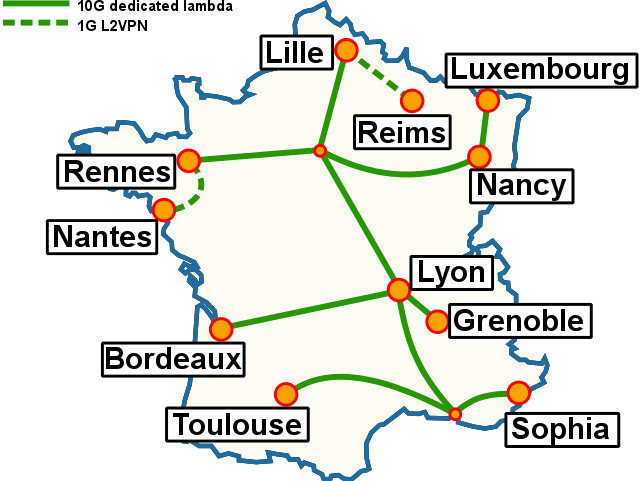
\includegraphics[scale=2]{./Figures/Renater5-g5k.jpg}
    \rule{35em}{0.5pt}
  \caption[Grid'5000 sites]{The sites of Grid'5000}
  \label{fig:g5ksites}
\end{figure}
It is very important with regard to the
experiments that inter-site communication and inter-node communication
are unrestricted and don't weigh any overhead on the
experiments. Thus, all communication can be done without any
constraints between sites. But
as for security, we have to take into account the following: if a
node is fully reconfigurable by the researcher, that means we
can't make any assumptions about the configuration of the security
mechanisms on an allocated node, thus, we have to assume that they are
unprotected. This is the reasoning behind the decision that sites
themselves (thus, of course, the nodes they are hosting) are not
directly connected to the Internet, making Grid'5000 an isolated
domain. This way, the sites are protected against DoS attacks.\\
It is possible to open restricted routes through the Internet to
external clusters, which provides the possibility of doing
multiplatform experiments.
\subsubsection{User view and data management}
As previously mentioned, communication is done with minimal
restrictions between Grid'5000 machines, meaning that authentication
procedures in such cases is also minimal: a user has a single account
across the whole platform. An LDAP directory is installed to provide
this in a reliable way. Every site runs an LDAP server. These servers
have the same root and there is a branch for every site. On a given
site, the local administrator has read-write access, as well as is
able to manage user accounts.\\
A user has access to all of the Grid'5000 sites and services
(monitoring tools, wiki, deployment, etc.). The user also has an
independent home directory at every site as well. Synchronization can
be done with any of the standard tools, such as \emph{rsync},
\emph{scp}, or \emph{sftp}. Data transfers to the outside world are
restricted - it can only be done via secure tools such as \emph{scp}
in order to prevent identity spoofing. Authentication is done via a
user-generated public key, in order to prevent brute-force attacks.
\subsubsection{Experiment scheduling}
\label{sec:experiment_scheduling}
At cluster level, the OAR\cite{xdghmmnr05} resource management system is
used to handle the scheduling of experiments and resource
allocation. Large-scale operations such as parallel task launching or
monitoring is handled by a specialized parallel launching tool,
Taktuk\cite{chr09}. Taktuk is a handy tool which can be used from the
console to, for example, perform a certain set of tasks on multiple
nodes.\\
A simple grid broker is handling resource management at grid
level, allowing co-allocation of nodes on multiple
clusters. Co-allocation is a very simple process for the user who,
after submitting an experiment needing several sets of nodes across
different clusters, receives an identifier from the broker which can
be used to retrieve all necessary information about the allocated
nodes.\\
Node reconfiguration, talked about in more detail below, co-operates
with the resource management system at certain points. Such a point is
that when a user submits an experiment that requires node
reconfiguration, the job submission is registered in a queue. Also, in
the prologue script that runs before the actual experiment, deployment
rights are given to the user which gives him/her the capability to
deploy system images on the allocated nodes. An epilogue script runs
after the experiment, revoking these rights. After the experiment is
finished, all of the allocated nodes are rebooted, deploying a default
environment, to provide a constant, unified system to run experiments
on that don't need node reconfiguration.
\subsubsection{Node reconfiguration}
Node reconfiguration on Grid'5000 is handled in a very user-friendly
way, using a tool called Kadeploy3\cite{jsn13}. For every user, a set
of default environments is available at start. After starting an
interactive job (that is, a job that requires node reconfiguration),
the user can deploy any of these environments by providing the chosen
image's name to Kadeploy3. Deployment usually takes only a few minutes
to complete - deployment time increases if we do the deployment on
more nodes. After this, the nodes are rebooted and the user can log
onto any of the nodes where an image was successfully deployed. When
logged in, the user can freely customize the environment: he/she can
install or remove software, modify configuration files, etc. - root
password is given to Grid'5000 users as well to provide more
possibilities. After reconfiguring the environment, the user has the
the possibility of saving the now customized image. This image
includes all software layers from OS to application levels, just as it
was for the default environments. The home directory is independent of
the image. After successfully saving an image, the user can deploy it
on the allocated nodes the same way he/she did for the default
images. This way, an environment tailored for the specific needs of
the user only needs to be created once, then it can be freely reused
on any other node on the site at a later time. When trying to port an
image created on one site to another site, there can be compatibility
issues due to inter-site differences. Modifications to the customized
image can be done with ease.
\section{An example process}
\label{sec:example_process}
To reiterate the more detailed description of trace acquisition, an
example process that we would like to automate consists of the
following steps, assuming that we already have a customized image set
up for our tests, as well as we already have an executable benchmark
application we'd like to run:
\begin{itemize}
\item allocate the specified number of nodes on a specified site
\item deploy our custom image on the allocated nodes
\item create a nodefile containing the names of the allocated nodes
\item broadcast the runnable across the nodes
\item disable all cores but one on every allocated node (see 3.4.1 for
  explanation)
\item run the mpi experiment from a chosen "head" node (can be any of
  the allocated nodes)
\item gather the traces from the allocated nodes to the head node
\item merge the traces
\item convert merged trace file to Paje format
\end{itemize}
As a side note: in this example, we assume that we are working on the
Grid'5000 testbed. As previously mentioned, most of the work regarding
this thesis was conducted there.\\
As for the example process: parameters that the user can give to it
are the number of nodes, the chosen Grid'5000 site, the image to
deploy, the runnable and parameters to mpirun (for example to disable
Infiniband) and the trace\_gather script. The nodefile created in the
3rd step is necessary for the operations that are needed to do
something on all the allocated nodes.\\
Now let's take a look at the experimentation engine we'd like to use
for implementing the framework to automate processes like this.
\section{XPflow}
XPflow is an experimentation engine, with one of its main goals being
to provide the possibility to easily automate experiments by creating
workflows. XPflow is a fairly new project. So new in fact, that at the
time of writing this thesis, its source code hasn't been published
yet, although it's going to be released in the very near future.
In 2.8.2, we already discussed business workflows, foreshadowing the
fact that XPflow, the tool used to implement our framework, is based
on that approach, which includes Business Process Modeling and
Management. There are 2 main concepts in XPflow\cite{bn12_2}:
\begin{itemize}
\item Process: It is the high-level description of the experiment,
  written in a DSL, which is embedded in Ruby. Processes are
  responsible for orchestrating activities and other processes,
  creating a workflow.
\item Activities: The low-level building blocks of the
  experiments. They are written in Ruby and used for implementing the
  lower-level details of the experiment, to do the "real work" in it
  (for example: manage files, start the MPI job).
\end{itemize}
Lets take a look at how these concepts are used through
examples, while uncovering a few other possibilities of XPflow.
\subsection{A general example}
First, we examine an example of transforming general, everyday
activities transformed into XPflow (\ref{fig:xpflow_example1}).
\begin{figure}[htbp]
  \centering
    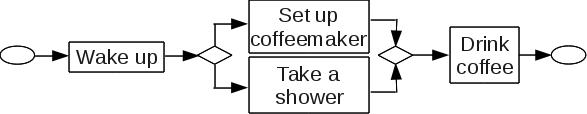
\includegraphics[scale=0.7]{./Figures/xpflow_example1.jpg}
  \caption[dayum]{Morning routine in XPflow}
  \label{fig:xpflow_example1}
\end{figure}
On the diagram, circles represent the starting and end point of the
process, the rectangles represent activities and the whole diagram
represents a process.\\
In XPflow, it is possible to execute activities sequentially or in
parallel. An example for sequential execution on
\ref{fig:xpflow_example1} is drinking coffee: the activities preceding
it must all be finished before that activity can be
started. On the contrary, setting up the coffeemaker and taking a
shower can be executed in parallel, since it's not necessary to stand
by the coffeemaker while it finishes - we can take a shower while it's
running.
\subsection{An MPI experiment example}
After the generic introduction, let's take a look at how we could
represent the experiment we described in section
\ref{sec:example_process} in XPflow. The representation can be seen on
\ref{fig:xpflow_example2}.
\begin{figure}[htbp]
  \centering
    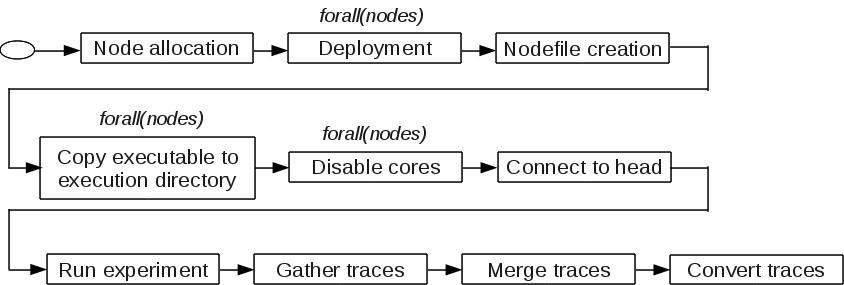
\includegraphics[scale=0.5]{./Figures/xpflow_example2.jpg}
  \caption[dayum]{An MPI experiment in XPflow}
  \label{fig:xpflow_example2}
\end{figure}
On this representation, there is no parallel execution like in the
previous example: one activity has to be executed sequentially after
the other, the activities depend on each other. However, as we can
see, some of the activities are distinguished by the text
"forall(nodes)" above them. This means that we iterate through all the
allocated nodes, executing the activity on all of them. This is done
in parallel.\\
As a side note: in the current implementation, this kind of iteration
is realized not
specifically by XPflow, but by the parallel launching tool mentioned
in \ref{sec:experiment_scheduling}, Taktuk\cite{chr09}. This is simply
because it was simpler to implement it that way, because this is a
known and stable solution, while XPflow is under heavy development
currently, thus its internals are subject to change. However, it could
be done with XPflow-specific funcionalities as well. In the long term,
using XPflow-specific funcionality would make the framework more
generic (less Grid'5000-specific).
\section{The framework}
In this section, we talk about the structure of the implemented
framework, its functionalities and usage.
The framework consists of two main parts: there is a frontend and
there is an XPflow structure called a "library" as a backend. While
the expression "library" may sound strange in this context, this is
what comes the closest to a class in XPflow: we are able to store
variables and have member functions, features which the framework
makes much use of.\\
Below is a more detailed discussion of the most important traits of
the frontend and the backend.
\subsection{Frontend}
The frontend is an interface between the user and the framework. It
has the function calls the user can use when orchestrating an
automated experiment. The example process in \ref{sec:example_process}
contains most of the processes that we'll discuss below.
\subsubsection{init; finish}
These processes need to be called at the
beginning and at the end of the experiment respectively. These methods
have tasks along the lines of variable initialization and metadata
collection. They will be discussed in greater detail when talking
about the backend.
\label{sec:keeping_of_nodes}
\subsubsection{reserve\_and\_deploy}
The allocation and deployment of
the nodes are in coupled inside one method, since it wouldn't make
sens to just start a job without deploying an operating system on the
allocated nodes. The framework currently only works with one specified
site, but the possibility to run experiments on nodes across multiple
sites could be implemented in the future. It's important to note that
when using XPflow's \emph{reserve\_nodes}, we set the \emph{keep
  =\textgreater  true} argument. This is so we actually keep the job
open until the
given time limit expires - we don't kill it at the end of the
experiment. This is so we can use \emph{checkpointing} (see below) to
run other experiments on the same nodes without having to do the
allocation and deployment process again (which can take up several
minutes).
\subsubsection{broadcast}
This method can be used to broadcast any file
across the nodes to a specified destination path. It can be utilized
to broadcast the benchmark runnable to every node to the destination
where the execution will take place. This needs to be done in order
for MPI to utilize all of the nodes - if a runnable is not present in
the place of execution on a given node, MPI won't be able to start its
processes there. For example, if we want to run the experiment and
generate the trace files in the /tmp directory, we will broadcast our
benchmark runnable to /tmp across the nodes.
\subsubsection{disable\_cores}
Disabling cores on nodes can be necessary
as a method to overcome simulation inaccuracy caused by SMPI's
inability to predict the performance of an MPI application when using
multiple cores, as mentioned before, in the \emph{Problem Description}
chapter.\\
This method, unlike the others in the frontend, is an \emph{activity}
instead of being a \emph{process}. This is done as a workaround to an
XPflow pitfall regarding proxy variables, an issue that will be
discussed in \ref{sec:proxy_variables}.
\subsubsection{mpirun}
This method is for actually running the benchmark
itself. It is important to give the full path to the mpirun runnable
as an argument to the process call, otherwise we can't be sure that
the MPI implementation running is the one we want.
\subsubsection{trace\_gather}
After running our MPI experiment, the gathered traces are scattered
amongst all the corresponding nodes. This process calls a script
called trace\_gather (which needs to be set up on the system image
manually), which copies the traces collected on the
different nodes to the one node we run the script on. We need to call
the script from the path where the execution happened, since that's
where the traces were gathered. After running
this process, we can assume that all the trace files are on the node
we made the function call from. For example if we have our traces in
/tmp, we need to call trace\_gather from there.
\subsubsection{merge\_traces}
This process calls the TAU\cite{sm06}
script \emph{tau\_treemerge.pl}, which is responsible for merging the
traces into one trace file. The script also tries to account for any
clock skew between the trace files with post-processing methods.\\
After we have one single trace file containing all our traces, we can
manipulate it easier: we can copy or move it, or convert it, for
example.
\subsection{Backend}
As mentioned before, the backend of the framework is an XPflow
construct called a \emph{library}. A library has state, so we can have
internal variables and methods, a functionality that we make use of:
if we couldn't save our state between individual function calls,
certain parameters, such as the number of nodes or the name of the
site we are working on would need to be given every time. Instead, we
can just put those values in variables and use them later when
needed.\\
Libraries can also contain activities. Most of the "real work" is put
into the library in the form of member activities. The backend
interfaces with the frontend, which makes calls to these activities
whenever needed.
\subsubsection{Metadata}
The backend library is also responsible for handling metadata
collection. Collected metadata includes:
\begin{itemize}
\item the date the experiment was run,
\item the runtime of the experiment,
\item the benchmark that was run,
\item the site and the nodes that were used for the experiment and
\item the image that was deployed on the nodes.
\end{itemize}
Certain elements of this list is provided by the user, while giving
certain parameters to a function call. For example when reserving
nodes, the user has to give the name of the site he/she wants to use,
as well as the name of the image that he/she wants to be
deployed. Other metadata is decided during runtime: a prime example to
this are the nodes used. The user only tells the framework the number
of nodes to allocate - the framework then gives the command on the
system to allocate the nodes, then saves the names of the allocated
nodes in a nodefile, which can be used later as a reference to our
nodes in question. There are also pieces of metadata directly
generated by the framework, such as the date and the runtime of the
experiment. The date is saved in the previously mentioned \emph{init}
method, while the runtime is calculated by saving the starting time in
the \emph{init} method, the ending time in the \emph{finish} method,
then calculating the difference.
\subsection{Checkpointing}
XPflow has a very useful feature, called checkpointing. A checkpoint
can be put anywhere in our experiment, making it possible that in the
next run, control is \emph{resumed} at the place of the checkpoint. An
example usage can be seen on \ref{fig:checkpoint1}: we put a
checkpoint after the allocation of nodes (line 12). As previously
mentioned in \ref{sec:keeping_of_nodes}, the node allocation is done
in such a way that they remain available even after the experiment is
done. So with putting a checkpoint there, we don't have to wait
through the several minute long node acquisition and deployment
process each time we want to run an MPI experiment: we can re-run it
on the same allocated nodes, as long as the time limit we set at the
node allocation allows us. It is also possible to change the code
after the checkpoint to run some other experiment, as it can be seen
on \ref{fig:checkpoint2}: there, we modify the code so it runs
\emph{dt.A.8} instead of \emph{lu.A.8}. We had to modify the code in
two places to achieve this: first, we need to broadcast the other
benchmark across the nodes (line 14) and the path to the runnable
needs to be changed as well when giving the command to run the
experiment (line 19). If the time interval we allocated the nodes for
passes, we have to run that part of the experiment again. This can be
done by telling XPflow to ignore the checkpoints (with the argument
\emph{-I}). In our example, this time interval is 30 minutes, as it
can be seen on line 10, where we give it as a parameter to the node
acquisition process.
\begin{figure}[htbp]
  \centering
    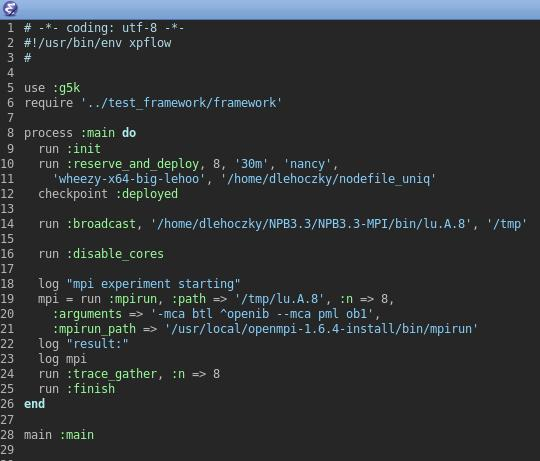
\includegraphics[scale=0.7]{./Figures/checkpoint1.jpg}
    \rule{35em}{0.5pt}
  \caption[Checkpoint example]{Example usage of checkpointing}
  \label{fig:checkpoint1}
\end{figure}
\begin{figure}[htbp]
  \centering
    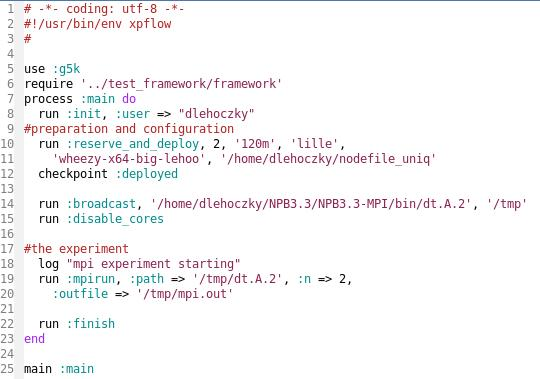
\includegraphics[scale=0.7]{./Figures/checkpoint2.jpg}
    \rule{35em}{0.5pt}
  \caption[Checkpoint example]{We can modify the code that comes after
  the checkpoint}
  \label{fig:checkpoint2}
\end{figure}
\subsection{Proxy variables}
\label{sec:proxy_variables}
There is a shortcoming of XPflow that caused a little headache during
the development of the framework. The problem stems from
the fact that the XPflow processes are written in a DSL that is
embedded in Ruby. Ruby is very
flexible in that regard, but one unsolved problem is that the body of
the process blocks are executed \emph{before} the execution of the
process itself. The problem with this is that at the time of the
execution of the process blocks, some of the variables that the
process uses contain only some proxy value, not the value that
was actually put in there. This problem has been briefly mentioned when
talking about the \emph{disable\_cores} method. In that particular
method, multiple command strings are needed, containing the commands
that are needed to be executed to disable the cores on the nodes. In
these command strings, the variable containing the nodefile is needed
to be inserted. If \emph{disable\_cores} was a process, this variable
would contain only a proxy variable at the
time we want to insert it in the string, even if we would put the
correct value in it right before. Writing this method as an activity
instead of a process solves this problem, since activities are written
in plain Ruby.
